\chapter{Software Testing and Validation} \label{chapter:testing}
% 在软件开发完成之后需要对软件进行测试以发现软件存在的错误和缺陷,进而对软件进行修补和完善,在测试完成之后需要对软件进行验证以检查软件表现是否符合需求文档的预期。
% 本文使用Mocha和Chai对项目的用户,市场,以及交易场景Api进行自动测试,通过模拟前端对后台的请求获得后台返回的数据,将返回的数据与预期的数据进行对比,如果数据一致则说明Api工作正确。自动测试结果如\fref{fig:testapi}所示,结果显示本项目的Api工作正常。
After the software is completed, the software needs to be tested to find bugs and defects, and then the software needs to be fixed and improved, followed by validation to check whether the software performs as expected in the requirements document. This chapter will display the result of testing and validation.

In this paper, Mocha and Chai are used to automatically test the Apis for user, market, and transaction scenarios of the project. The result of the automatic test is shown in \fref{fig:testapi}.
\begin{figure}[!htb]
    \centering
    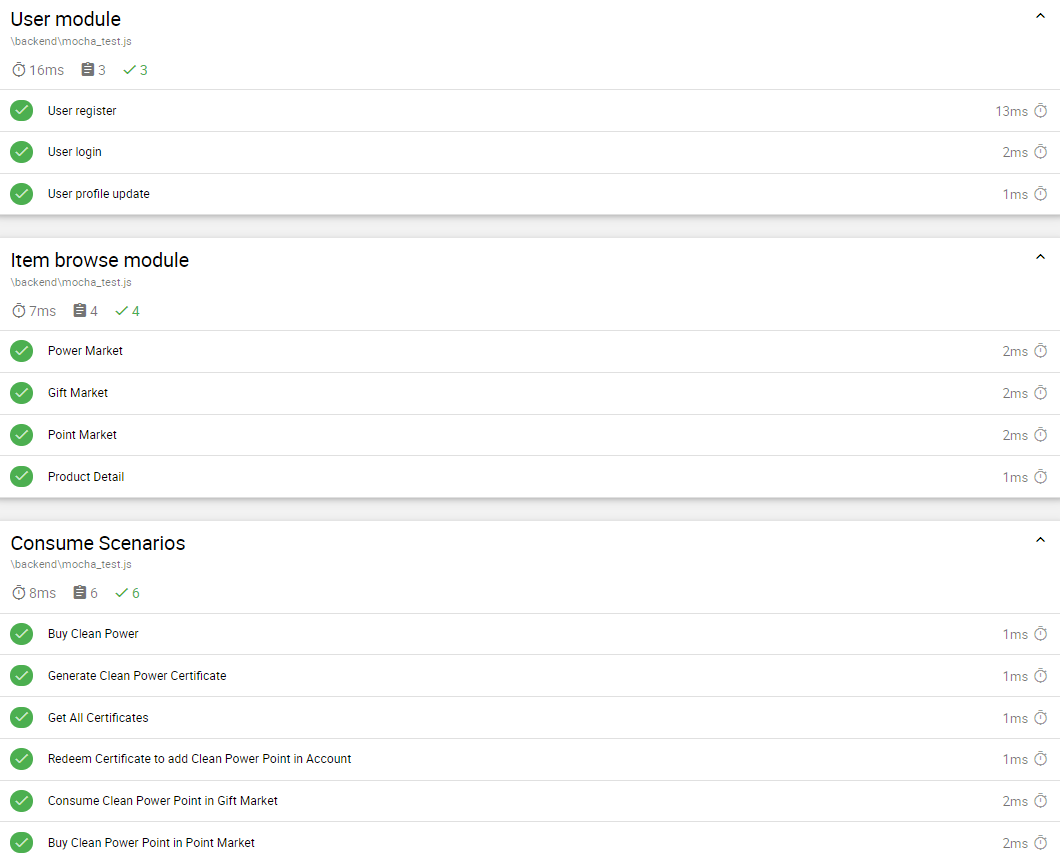
\includegraphics[width=.8 \textwidth]{img/testresult.png}
    \caption{Testing result of Apis}
    \label{fig:testapi}
\end{figure}

% 本文通过Hyper Ledger Explorere进行软件验证,在每一项操作完成之后对区块链数据进行查看,\fref{fig:dataoverview}和\fref{fig:transaction}分别代表了区块链数据总览以及交易信息查看,验证结果显示本项目符合需求文档要求。
Hyper Ledger Explorere is used to validate the software in this project, and the blockchain data is viewed after each operation is completed, \fref{fig:dataoverview} and \fref{fig:transaction} represent the blockchain data overview and transaction information view respectively. The validation results show that this project meets the requirements of the requirement document.
\begin{figure}[!htb]
    \centering
    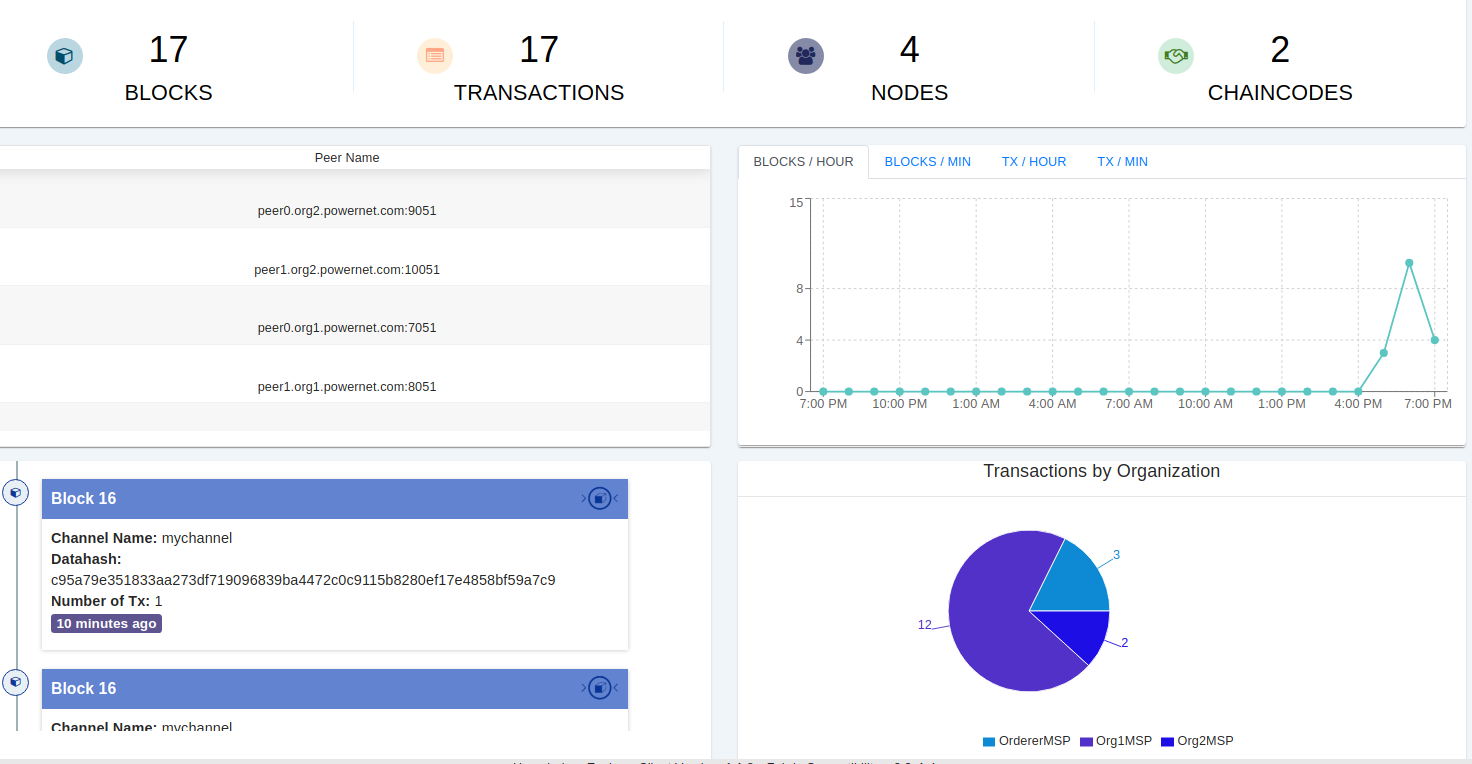
\includegraphics[width= \textwidth]{img/overview.png}
    \caption{System data overview}
    \label{fig:dataoverview}
\end{figure}
\begin{figure}[!htb]
    \centering
    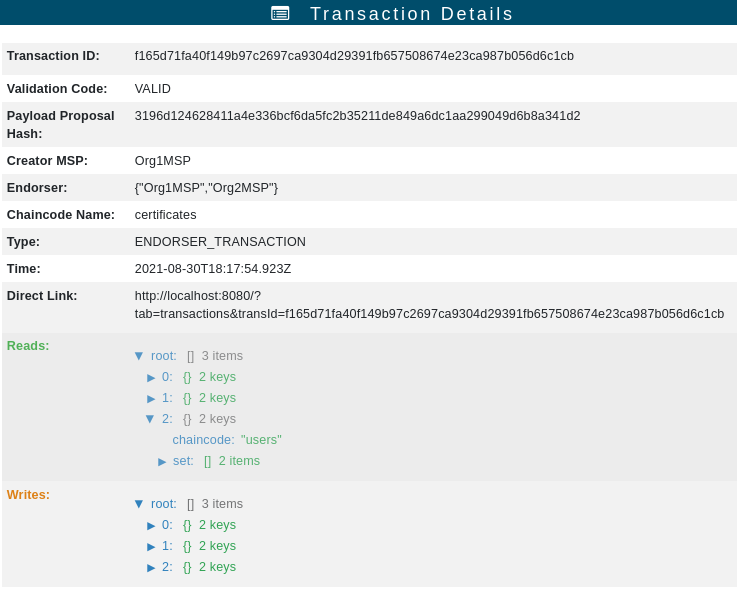
\includegraphics[width=.9 \textwidth]{img/transaction.png}
    \caption{Transaction monitoring}
    \label{fig:transaction}
\end{figure}
